\documentclass[12pt,a4paper]{article}
\usepackage[margin=1in]{geometry}
\usepackage{amsmath,booktabs,hyperref,enumitem,xcolor,listings,tikz}
\usetikzlibrary{positioning,arrows.meta}
\lstset{language=Python,basicstyle=\ttfamily\small,keywordstyle=\color{blue},commentstyle=\color{gray},showstringspaces=false,breaklines=true,frame=single}
\title{Neural Network and Deep Learning\\Assignment Question 3}
\author{}\date{}
\begin{document}\maketitle
\section*{3. Convolutional Neural Networks and VGG Architecture}
\subsection*{CNN principles}
A convolutional neural network exploits the fact that nearby pixels are related and that a useful pattern can occur at different locations. A small learnable filter (kernel) slides over an image. At each position it computes a weighted sum plus bias, producing one entry of a feature map:
\[
S(i,j)=\sum_{u,v,c}K(u,v,c)X(i+u,j+v,c)+b.
\]
Many filters learn edges, corners, textures, and eventually object parts. ReLU, $\max(0,z)$, supplies nonlinearity. Padding preserves spatial dimensions; stride controls the step size. Max or average pooling reduces spatial resolution and makes representations less sensitive to small translations. Fully connected layers combine high-level features for classification, while softmax converts logits into class probabilities.

\begin{center}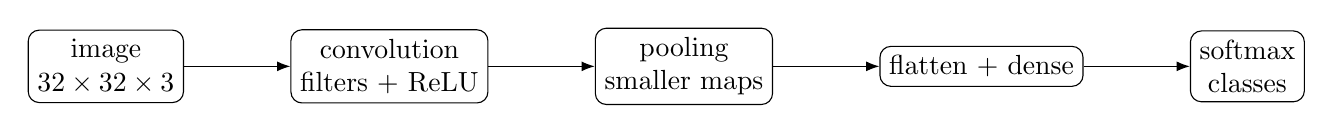
\begin{tikzpicture}[node distance=1.35cm,>=Latex, every node/.style={draw,rounded corners,align=center}]
\node (i) {image\\$32\times32\times3$};\node[right=of i](c){convolution\\filters + ReLU};\node[right=of c](p){pooling\\smaller maps};\node[right=of p](f){flatten + dense};\node[right=of f](o){softmax\\classes};
\draw[->](i)--(c);\draw[->](c)--(p);\draw[->](p)--(f);\draw[->](f)--(o);
\end{tikzpicture}\end{center}

\subsection*{VGG16 and VGG19}
VGG networks use a deliberately simple pattern: repeated $3\times3$ convolutions with stride 1 and padding, ReLU after each convolution, then $2\times2$ max pooling with stride 2. Five convolutional blocks progressively reduce width and height while increasing channels from 64 to 512. After flattening, the original ImageNet models use two 4096-unit dense layers and a 1000-class output.
\begin{center}\begin{tabular}{lcc}\toprule
Block & VGG16 convolutions & VGG19 convolutions\\\midrule
1 & 2 $\times$ 64 & 2 $\times$ 64\\
2 & 2 $\times$ 128 & 2 $\times$ 128\\
3 & 3 $\times$ 256 & 4 $\times$ 256\\
4 & 3 $\times$ 512 & 4 $\times$ 512\\
5 & 3 $\times$ 512 & 4 $\times$ 512\\\bottomrule
\end{tabular}\end{center}
\begin{center}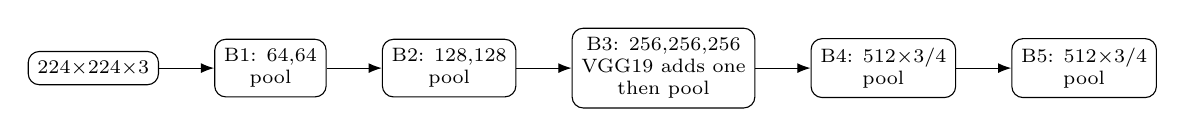
\begin{tikzpicture}[node distance=7mm,>=Latex, every node/.style={draw,rounded corners,align=center,font=\scriptsize}]
\node(a){224$\times$224$\times$3};\node[right=of a](b){B1: 64,64\\pool};\node[right=of b](c){B2: 128,128\\pool};\node[right=of c](d){B3: 256,256,256\\VGG19 adds one\\then pool};\node[right=of d](e){B4: 512$\times$3/4\\pool};\node[right=of e](f){B5: 512$\times$3/4\\pool};\draw[->](a)--(b);\draw[->](b)--(c);\draw[->](c)--(d);\draw[->](d)--(e);\draw[->](e)--(f);\end{tikzpicture}\end{center}
Consecutive $3\times3$ filters have effective receptive field $5\times5$ or $7\times7$ with fewer parameters than one large filter, and insert extra ReLU nonlinearities. Stride 1 with same padding preserves dimensions before each $2\times2$ stride-2 pool; pooling halves width and height.
Both have five pooling operations. VGG16 has 13 convolutional layers and 16 weight layers; VGG19 has 16 convolutional and 19 weight layers. VGG19 can represent more complex features but costs more memory and computation. Modern models may outperform VGG, but VGG remains useful for teaching and feature extraction.

\subsection*{Simple CNN implementation}
\begin{lstlisting}
import tensorflow as tf
from tensorflow.keras import layers, Sequential

(x_train, y_train), (x_test, y_test) = tf.keras.datasets.mnist.load_data()
x_train = x_train[..., None].astype("float32") / 255.0
x_test = x_test[..., None].astype("float32") / 255.0
model = Sequential([
    layers.Input((28, 28, 1)), layers.Conv2D(32, 3, activation="relu"),
    layers.MaxPooling2D(), layers.Conv2D(64, 3, activation="relu"),
    layers.MaxPooling2D(), layers.Flatten(), layers.Dense(64, "relu"),
    layers.Dense(10, "softmax")])
model.compile("adam", "sparse_categorical_crossentropy", metrics=["accuracy"])
model.fit(x_train, y_train, epochs=3, batch_size=128, validation_split=.1, verbose=2)
print(model.evaluate(x_test, y_test, verbose=0))
\end{lstlisting}
Pixels are reshaped to add the channel dimension and scaled to $[0,1]$. \texttt{Conv2D} learns 32 and then 64 spatial filters. Pooling halves the map dimensions. \texttt{Flatten} changes maps into a vector, and the dense layers classify ten digits. Sparse cross-entropy accepts integer labels. A typical output is validation accuracy about 0.99 and test accuracy about 0.99; the exact value depends on hardware and random initialisation. High test accuracy indicates that learned local features transfer from training digits to unseen digits.

\subsection*{Pre-trained VGG feature extraction}
\begin{lstlisting}
from tensorflow.keras.applications import VGG16
from tensorflow.keras.applications.vgg16 import preprocess_input, decode_predictions
from tensorflow.keras.utils import load_img, img_to_array
import numpy as np

vgg = VGG16(weights="imagenet", include_top=True)
image = load_img("sample.jpg", target_size=(224, 224))
batch = preprocess_input(img_to_array(image)[None, ...])
probabilities = vgg.predict(batch, verbose=0)
print(decode_predictions(probabilities, top=3)[0])

extractor = VGG16(weights="imagenet", include_top=False, pooling="avg")
features = extractor.predict(batch, verbose=0)
print(features.shape)
\end{lstlisting}
\texttt{weights="imagenet"} downloads learned weights once. VGG expects $224\times224$ RGB input, and \texttt{preprocess\_input} applies the same channel preprocessing used during training. With \texttt{include\_top=True}, \texttt{decode\_predictions} maps the 1000 probabilities to readable labels. With \texttt{include\_top=False}, the classifier is removed; global average pooling returns a 512-dimensional feature vector suitable for nearest-neighbour search or a small downstream classifier. A representative result is three labels with probabilities summing below one because only the top three are printed, followed by \texttt{(1, 512)}. The program requires an image file and network access on the first weight download.
\end{document}